\PassOptionsToPackage{table}{xcolor}

\documentclass[
%	handout,
	notes=none,
	aspectratio=169
]{beamer}

% Comment out the following line to hide the notes
%\setbeameroption{show notes}

% Imports
\usepackage{listings}
\usepackage{amsfonts}
\usepackage{amsmath}
\usepackage{pythonhighlight}
\usepackage{pgfpages}
\usepackage{tabularx}
\usepackage{ifxetex,ifluatex}
\usepackage{etoolbox}
\usepackage{framed}

\mode<handout>{%
	\pgfpagesuselayout{8 on 1}[a4paper,border shrink=5mm]
	\setbeameroption{show notes}
}

% Graphics configuration
\graphicspath{{./graphics/}}
\DeclareGraphicsExtensions{.pdf,.jpeg,.png,.jpg,.pdf}

% Useful macros
\def\etal{{\it et al.}}
\def\etc{{\it etc.}}
\def\eg{{\it e.g.}}
\def\ie{{\it i.e.}}
\def\cf{{\it cf.}}
\def\qv{{\it q.v.}}
\def\qqv{{\it qq.v.}}
\def\st{s.t.\ }
\def\code{\tt}
\def\setsep{:}
\def\concat{\mathbin{|}}

\renewcommand{\thefootnote}{\fnsymbol{footnote}}
\newcommand{\prescite}[1]{\footnote{\cite{#1}}}
\newcommand{\prestext}[1]{\footnotetext{\cite{#1}}}
\newcommand{\emaillink}[1]{\href{mailto:#1}{\nolinkurl{#1}}}

\setlength{\parskip}{0.5em}

% Tables

\newcolumntype{L}[1]{>{\raggedright\arraybackslash\tiny}p{#1}}

% Program listings
\definecolor{listingbaground}{rgb}{.9,.9,.9}

\lstset{
	language=C,
	backgroundcolor=\color{listingbaground},
	extendedchars=true,
	basicstyle=\fontsize{5pt}{6pt}\ttfamily,
	showstringspaces=false,
	showspaces=false,
	numbers=left,
	numberstyle=\fontsize{5pt}{6pt}\ttfamily\color{gray},
	numbersep=5pt,
	tabsize=2,
	breaklines=true,
	showtabs=false,
	captionpos=b,
	xleftmargin=5mm,
	escapeinside={££}{££},
	framexleftmargin=5mm,
	showlines=true
}

% https://tex.stackexchange.com/questions/89574/language-option-supported-in-listings
\lstdefinelanguage{JavaScript}{
	keywords={typeof, new, true, false, catch, function, return, null, catch, switch, var, if, in, while, do, else, case, break},
	keywordstyle=\color{blue}\bfseries,
	ndkeywords={class, export, boolean, throw, implements, import, this},
	ndkeywordstyle=\color{darkgray}\bfseries,
	identifierstyle=\color{black},
	sensitive=false,
	comment=[l]{//},
	morecomment=[s]{/*}{*/},
	commentstyle=\color{purple}\ttfamily,
	stringstyle=\color{red}\ttfamily,
	morestring=[b]',
	morestring=[b]"
}

\lstdefinelanguage{QML}{
	keywords={typeof, new, true, false, catch, function, return, null, catch, switch, var, if, in, while, do, else, case, break, id, property, bool, string, int, decimal, target},
	keywordstyle=\color{blue}\bfseries,
	ndkeywords={Page, Example, Timer, Column, PageHeader, TextSwitch, Label},
	ndkeywordstyle=\color{teal}\bfseries,
	identifierstyle=\color{black},
	sensitive=true,
	comment=[l]{//},
	morecomment=[s]{/*}{*/},
	commentstyle=\color{green}\ttfamily,
	stringstyle=\color{red}\ttfamily,
	morestring=[b]',
	morestring=[b]"
}

\lstdefinelanguage{cpp}{
	keywords={class, public, private, try, throw, catch, this, return, null, switch, if, while, do, else, case, break, for, bool, void, const, static, volatile, int},
	keywordstyle=\color{blue}\bfseries,
	ndkeywords={Q_OBJECT, Q_CLASSINFO, Q_PROPERTY, Q_SLOTS, Q_SIGNALS, signals, slots, READ, WRITE, NOTIFY, QString, QUrl, CefString, CefRefPtr, qreal},
	ndkeywordstyle=\color{teal}\bfseries,
	identifierstyle=\color{black},
	sensitive=false,
	comment=[l]{//},
	morecomment=[s]{/*}{*/},
	commentstyle=\color{purple}\ttfamily,
	stringstyle=\color{red}\ttfamily,
	morestring=[b]',
	morestring=[b]"
}

\lstdefinelanguage{sh2}{
	keywords={dbus, send, zypper, python3},
	keywordstyle=\color{blue}\bfseries,
	ndkeywords={session, type, print, reply, dest},
	ndkeywordstyle=\color{teal}\bfseries,
	identifierstyle=\color{black},
	sensitive=false,
	comment=[l]{\#},
	morecomment=[s]{/*}{*/},
	commentstyle=\color{purple}\ttfamily,
	stringstyle=\color{red}\ttfamily,
	morestring=[b]',
	morestring=[b]"
}

% To allow the theme files to be placed in a subdirectory
\makeatletter
	\def\beamer@calltheme#1#2#3{%
		\def\beamer@themelist{#2}
		\@for\beamer@themename:=\beamer@themelist\do
		{\usepackage[{#1}]{\beamer@themelocation/#3\beamer@themename}}}

	\def\usefolder#1{
		\def\beamer@themelocation{#1}
	}
	\def\beamer@themelocation{}

% Quotation styling
% conditional for xetex or luatex
\newif\ifxetexorluatex
\ifxetex
  \xetexorluatextrue
\else
  \ifluatex
    \xetexorluatextrue
  \else
    \xetexorluatexfalse
  \fi
\fi
%
\ifxetexorluatex%
  \usepackage{fontspec}
  \newfontfamily\quotefont[Ligatures=TeX]{Source Sans Pro} % selects Libertine as the quote font
\else
  \usepackage[utf8]{inputenc}
  \usepackage[T1]{fontenc}
  \newcommand*\quotefont{\fontfamily{Source Sans Pro}} % selects Libertine as the quote font
\fi

\newcommand*\quotesize{60} % if quote size changes, need a way to make shifts relative
% Make commands for the quotes
\newcommand*{\openquote}
   {\tikz[remember picture,overlay,xshift=-3ex,yshift=-2.5ex]
   \node (OQ) {\quotefont\fontsize{\quotesize}{\quotesize}\selectfont``};\kern0pt}

\newcommand*{\closequote}[1]
  {\tikz[remember picture,overlay,xshift=3ex,yshift={#1}]
   \node (CQ) {\quotefont\fontsize{\quotesize}{\quotesize}\selectfont''};}

% select a colour for the shading
\definecolor{shadecolor}{HTML}{ffffff}

\newcommand*\shadedauthorformat{\emph} % define format for the author argument

% Now a command to allow left, right and centre alignment of the author
\newcommand*\authoralign[1]{%
  \if#1l
    \def\authorfill{}\def\quotefill{\hfill}
  \else
    \if#1r
      \def\authorfill{\hfill}\def\quotefill{}
    \else
      \if#1c
        \gdef\authorfill{\hfill}\def\quotefill{\hfill}
      \else\typeout{Invalid option}
      \fi
    \fi
  \fi}
% wrap everything in its own environment which takes one argument (author) and one optional argument
% specifying the alignment [l, r or c]
%
\newenvironment{shadequote}[2][l]%
{\authoralign{#1}
\ifblank{#2}
   {\def\shadequoteauthor{}\def\yshift{-2ex}\def\quotefill{\hfill}}
   {\def\shadequoteauthor{\par\authorfill\shadedauthorformat{#2}}\def\yshift{2ex}}
\begin{snugshade}\begin{quote}\openquote}
{\shadequoteauthor\quotefill\closequote{\yshift}\end{quote}\end{snugshade}}




\usefolder{theme}
\usetheme{sailfish}

\begin{document}

\title{Anatomy of a Browser}
\subtitle{Embedded Mobile Lizards}
\author{David Llewellyn-Jones}
\date{5th November 2024}

%%%%%%%%%%%%%%%%%%%%%%%%%%%%%%%%%%%%%%%%%

\renewcommand{\thefootnote}{\arabic{footnote}}

\frame{
\titlepage
}
\note{
}

\renewcommand{\thefootnote}{\fnsymbol{footnote}}

%%%%%%%%%%%%%%%%%%%%%%%%%%%%%%%%%%%%%%%%%

\begin{frame}
\frametitle{Gecko}

\begin{columns}[T]
\begin{column}[T]{0.6\textwidth}
\setlength{\parskip}{0.5em}

\vspace{1.5cm}
\begin{enumerate}
\setlength{\parskip}{0.5em}
\item Mozilla's rendering engine used in Firefox
\item Released in 2000, Netscape 6
\item Alternative to Blink, WebKit, Netsurf
\end{enumerate}

\end{column}
\begin{column}[T]{0.4\textwidth}
\setlength{\parskip}{0.5em}

\vspace{0.5cm}

\includegraphics[width=1.0\textwidth]{mozilla}

\end{column}
\end{columns}

\end{frame}
\note{
\begin{enumerate}
\item Mozilla's rendering engine used in Firefox
\item First appeared in 2000 with the release of Netscape 6
\item Alternative to Blink (Chrome, Edge, Brave, Vivaldi), WebKit (Safari, iOS, Ephiphany), Netsurf (Netsurf)
\end{enumerate}
}

%%%%%%%%%%%%%%%%%%%%%%%%%%%%%%%%%%%%%%%%%

\begin{frame}
\frametitle{Embedded Browsers}

\begin{columns}[T]
\begin{column}[T]{1.0\textwidth}
\setlength{\parskip}{0.5em}

\vspace{0.5cm}

\begin{shadequote}[r]{WPE, October 2024}
For many of us, a browser is an application... You click an icon on your graphical operating system, navigate somewhere with a URL bar, search, and so on... In contrast, an \textbf{\textit{embedded browser}} is contained within another application or is built for a specific purpose and runs in an embedded system, and the application controlling the embedded browser does not provide all the typical features of browsers running in desktops.
\end{shadequote}

\end{column}
\end{columns}

\end{frame}
\note{
WPE: Web Platform for Embedded

What is an Embedded Browser?

\url{https://wpewebkit.org/about/what-is-embedded.html}
}

%%%%%%%%%%%%%%%%%%%%%%%%%%%%%%%%%%%%%%%%%

\begin{frame}
\frametitle{Embedded Browsers}

\begin{columns}[T]
\begin{column}[T]{0.55\textwidth}
\setlength{\parskip}{0.5em}

\vspace{1.5cm}
What does ``embedded'' mean?
\begin{enumerate}
\setlength{\parskip}{0.5em}
\item Smaller resource footprint devices
\item Embeddable in other programs
\item Minimal user interface
\item All of the above
\end{enumerate}

\end{column}
\begin{column}[T]{0.37\textwidth}
\setlength{\parskip}{0.5em}

\vspace{1.0cm}

\includegraphics[width=0.9\textwidth]{mozilla-on-sailfish}

\end{column}
\end{columns}

\end{frame}
\note{
\begin{enumerate}
\item -
\end{enumerate}
}

%%%%%%%%%%%%%%%%%%%%%%%%%%%%%%%%%%%%%%%%%

\begin{frame}
\frametitle{}

\begin{columns}[T]
\begin{column}[T]{1.05\textwidth}

\vspace{0.7cm}
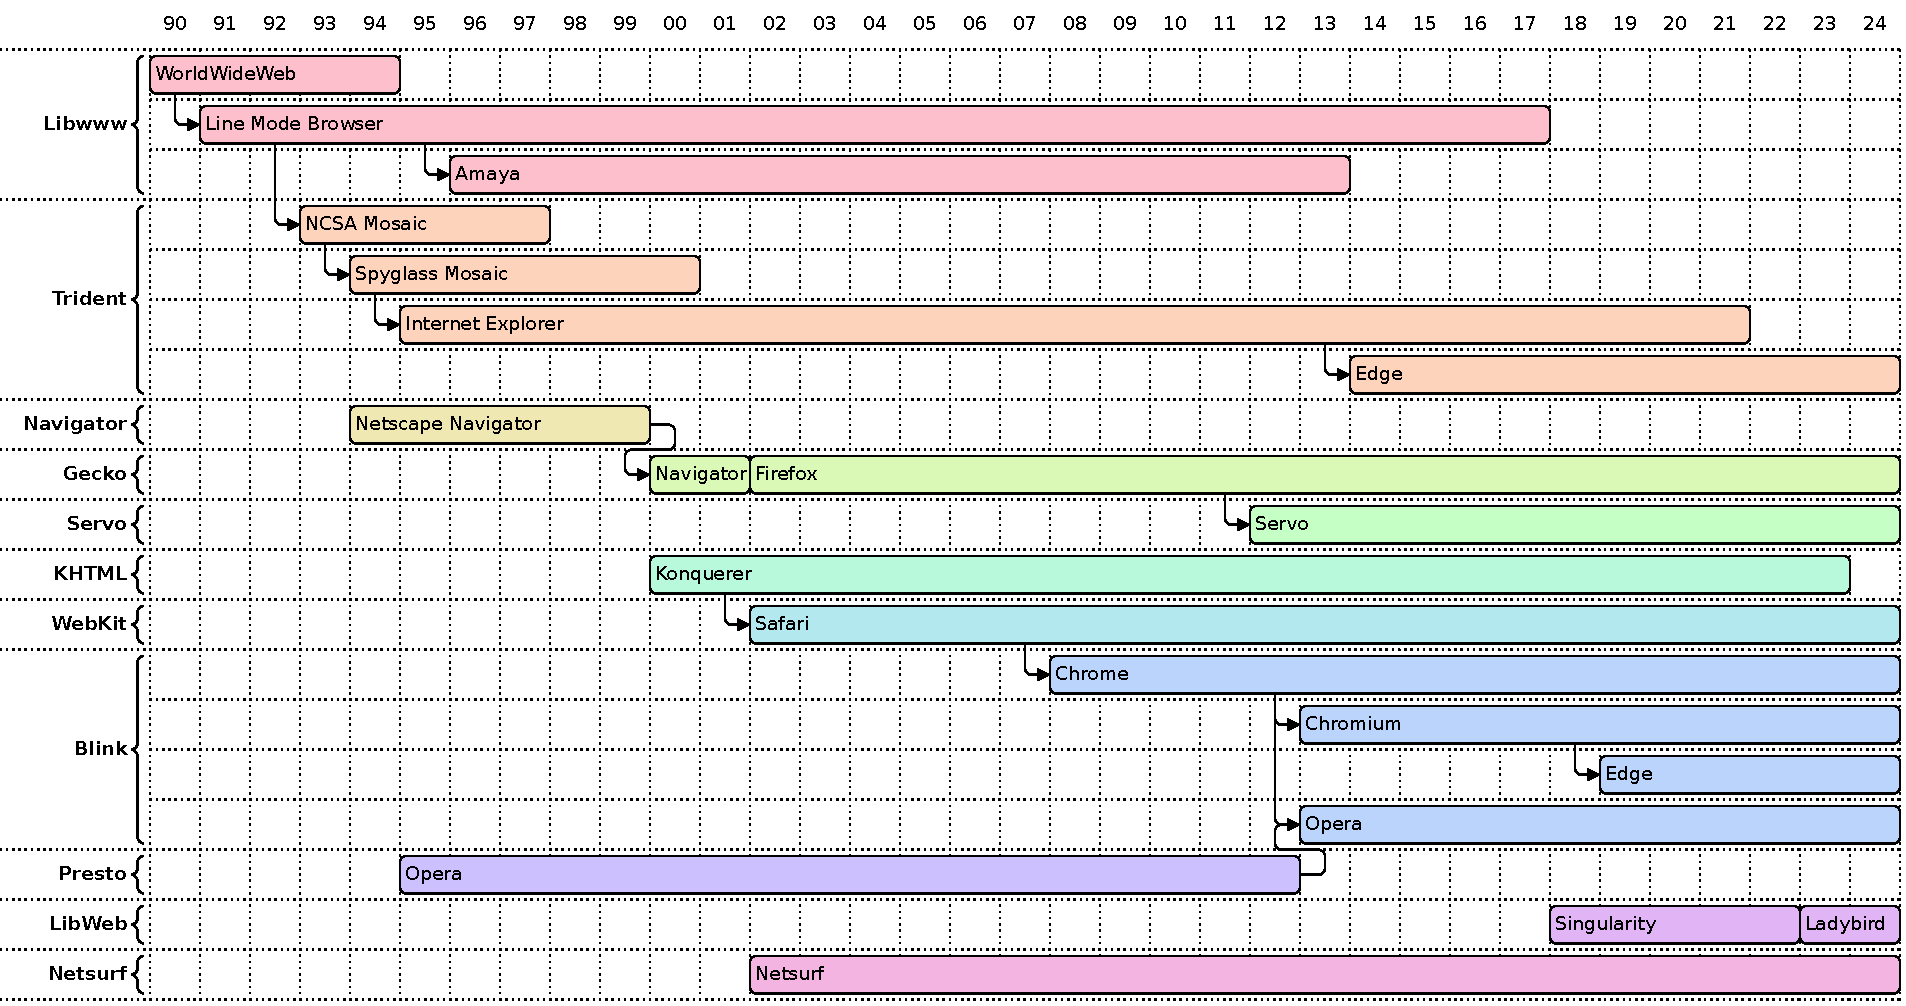
\includegraphics[width=1.0\textwidth]{gantt}

\end{column}
\end{columns}

\end{frame}
\note{
\begin{enumerate}
\item The browser history timeline.
\end{enumerate}
}

%%%%%%%%%%%%%%%%%%%%%%%%%%%%%%%%%%%%%%%%%

\begin{frame}
\frametitle{Embedding Gecko}

\begin{columns}[T]
\begin{column}[T]{1.0\textwidth}
\setlength{\parskip}{0.5em}

\vspace{0.5cm}

\begin{shadequote}[r]{Chris Lord, February 2016}
Gecko has limited embedding capability that is not well-documented, not well-maintained and not heavily invested in... We have at various points in history had embedding APIs/capabilities, but we have either dropped them (gtkmozembed) or let them bit-rot (IPCLite).
\end{shadequote}

\end{column}
\end{columns}

\end{frame}
\note{
\begin{enumerate}
\item It's an old quote, but holds true today.
\item Chris Lord was a Mozilla engineer at the time.
\item He makes clear he's not criticising the implementations, but rather the strategic direction of Mozilla.
\item IPCLite is another name for EmbedLite.
\item \url{https://www.chrislord.net/2016/02/24/the-case-for-an-embeddable-gecko/}
\item \url{https://www.chrislord.net/2016/03/08/state-of-embedding-in-gecko/}
\end{enumerate}
}

%%%%%%%%%%%%%%%%%%%%%%%%%%%%%%%%%%%%%%%%%

\begin{frame}
\frametitle{Context}

\begin{columns}[T]
\begin{column}[T]{0.7\textwidth}
\setlength{\parskip}{0.5em}

\vspace{2.0cm}
\begin{enumerate}
\setlength{\parskip}{0.5em}
\item Work upgrading the browser on Sailfish OS
\item ESR 78.15.0 to ESR 91.9.1
\item Work conducted over 13 months: August 2023 - September 2024
\end{enumerate}

\end{column}
\begin{column}[T]{0.3\textwidth}
\setlength{\parskip}{0.5em}

\vspace{0.5cm}


\vspace{0.5cm}
{\centering


\includegraphics[width=0.95\textwidth]{qrcode-gecko-dev}

\vspace{-0.1cm}

\noindent{\parbox{0.8\textwidth}{{\large
\href{https://www.flypig.co.uk/gecko}{{\tt https:// \\
www.flypig.co.uk \\
/gecko\\
}}
}}
}


}

\end{column}
\end{columns}

\end{frame}
\note{
\begin{enumerate}
\item -
\end{enumerate}
}

%%%%%%%%%%%%%%%%%%%%%%%%%%%%%%%%%%%%%%%%%

\begin{frame}
\frametitle{}

\begin{columns}[T]
\begin{column}[T]{1.13\textwidth}

\vspace{0.0cm}
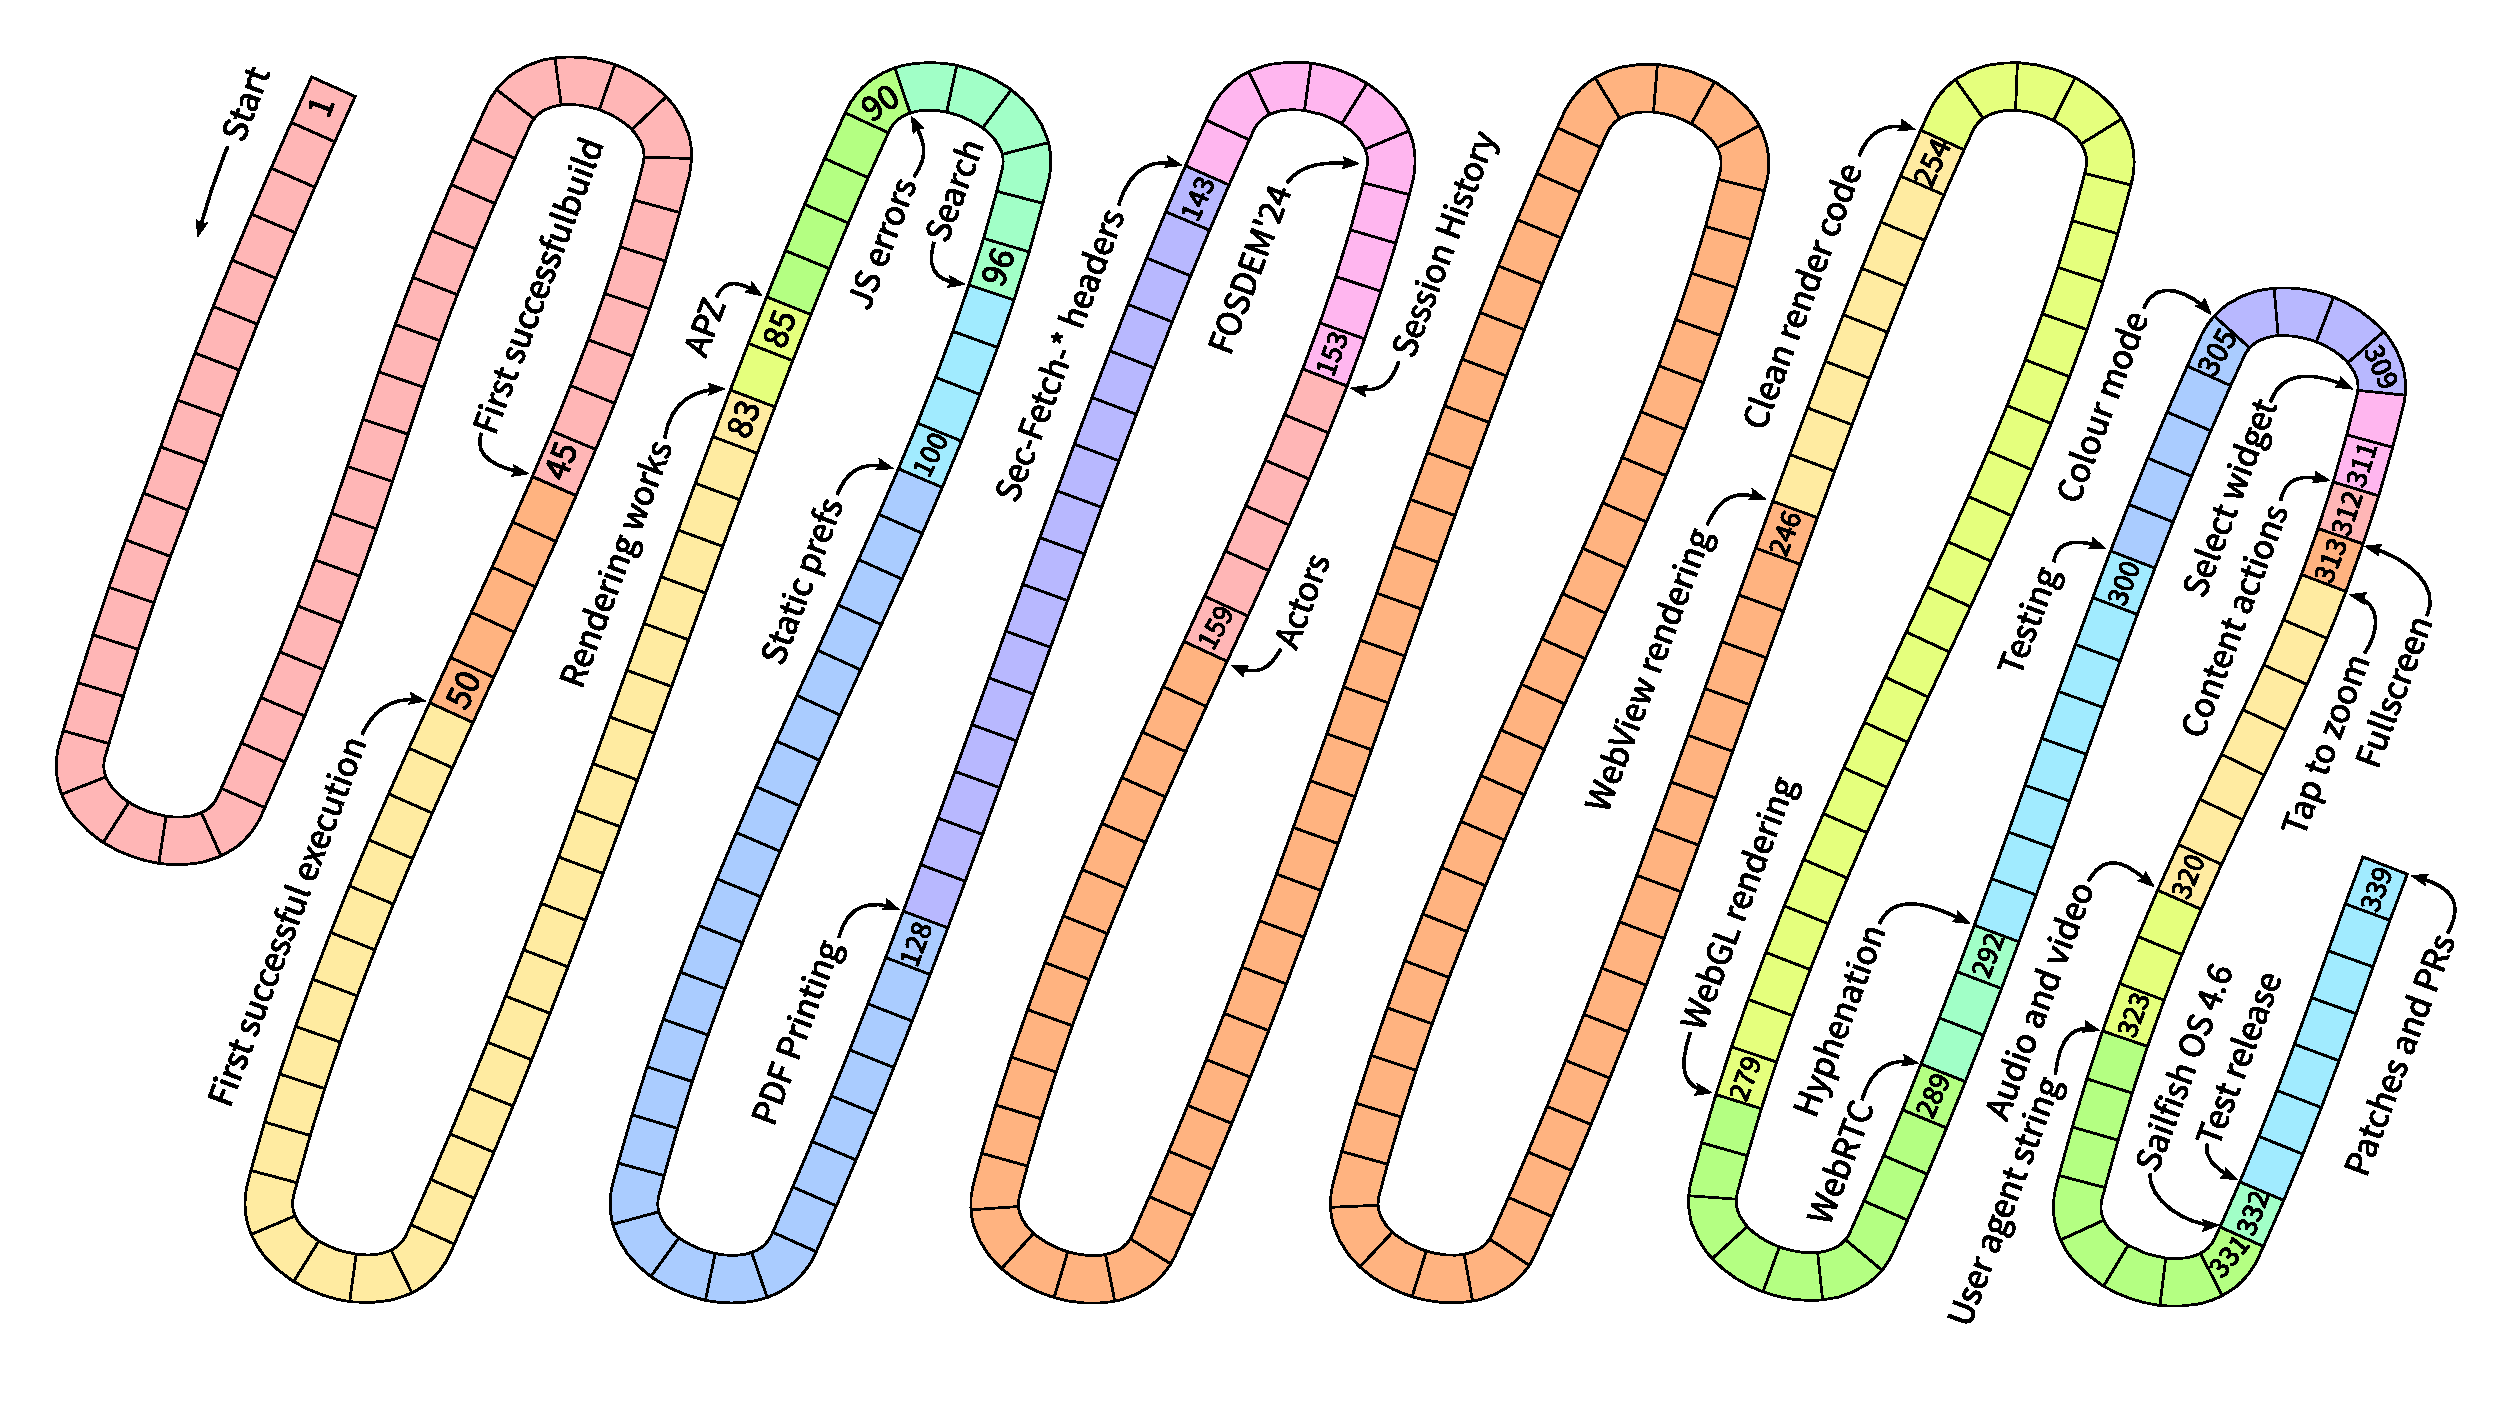
\includegraphics[width=1.0\textwidth]{timeline-dev}

\end{column}
\end{columns}

\end{frame}
\note{
\begin{enumerate}
\item The timeline of work up until now.
\end{enumerate}
}

%%%%%%%%%%%%%%%%%%%%%%%%%%%%%%%%%%%%%%%%%

\begin{frame}
\frametitle{Challenges working with the browser}

\begin{columns}[T]
\begin{column}[T]{0.5\textwidth}
\setlength{\parskip}{0.5em}

\vspace{1.5cm}
\begin{enumerate}
\setlength{\parskip}{0.5em}
\item Long build times
\item Complex build process
\item Random upstream changes (e.g. converting quote characters)
\item Removal of the entire EmbedLite rendering pipeline
\end{enumerate}

\end{column}
\begin{column}[T]{0.5\textwidth}
\setlength{\parskip}{0.5em}

\vspace{0.5cm}

\includegraphics[width=1.0\textwidth]{mozilla}

\end{column}
\end{columns}

\end{frame}
\note{
\begin{enumerate}
\item -
\end{enumerate}
}

%%%%%%%%%%%%%%%%%%%%%%%%%%%%%%%%%%%%%%%%%

\begin{frame}
\frametitle{Sailfish Browser}

\begin{columns}[T]
\begin{column}[T]{1.1\textwidth}

\vspace{0.5cm}
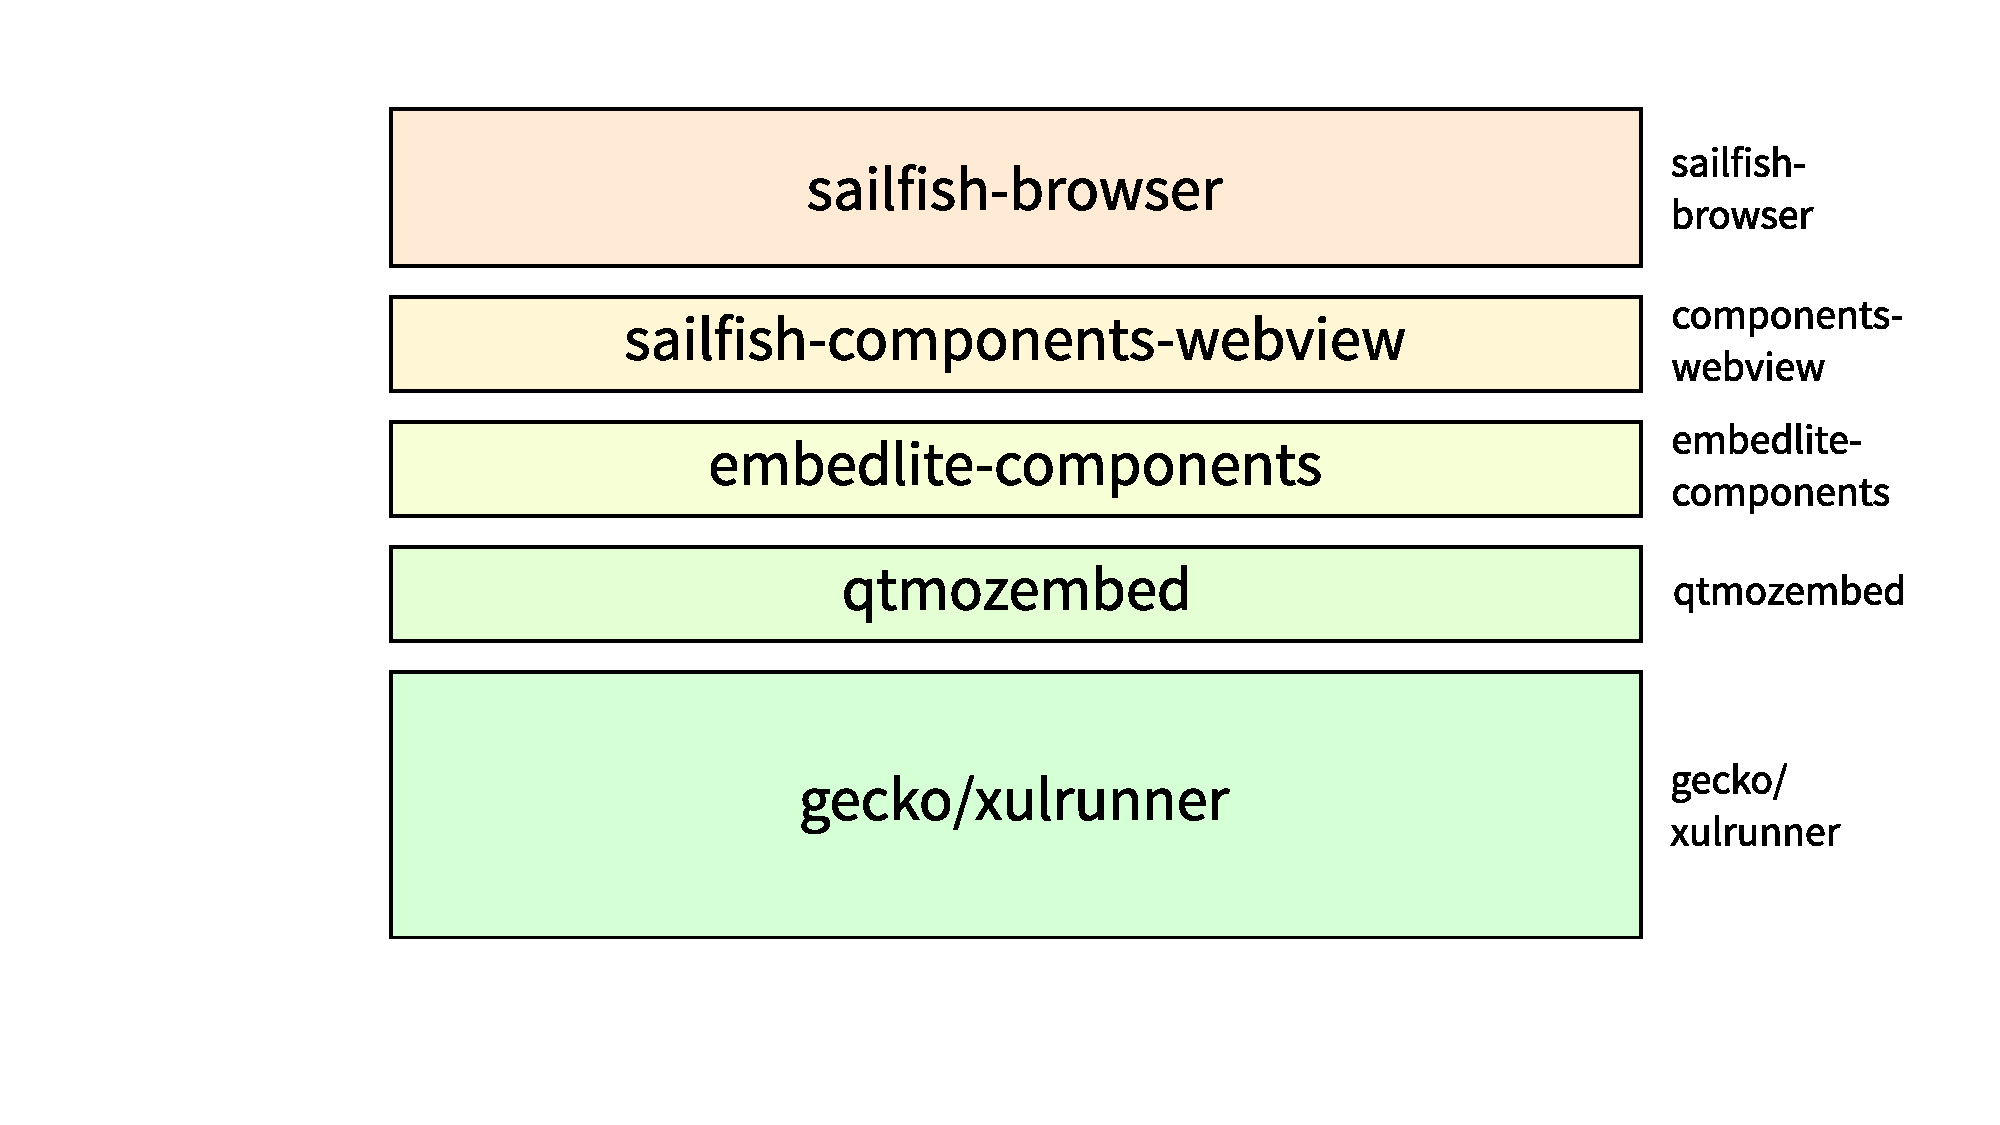
\includegraphics[width=1.0\textwidth]{components}

\end{column}
\end{columns}

\end{frame}
\note{
\begin{enumerate}
\item The Sailfish Browser isn't just gecko.
\item {\tt sailfish-browser} provides the user interface (C++/Qt/QML).
\item {\tt embedlite-components} provides JavaScript user interface functionality (JavaScript).
\item {\tt qtmozembed} turns gecko into an embeddable Qt component (C++/Qt).
\item {\tt gecko} is the EmbedLite embedded gecko renderer (JavaScript/C++/Rust).
\end{enumerate}
}

%%%%%%%%%%%%%%%%%%%%%%%%%%%%%%%%%%%%%%%%%

\begin{frame}
\frametitle{Sailfish Browser}

\begin{columns}[T]
\begin{column}[T]{1.1\textwidth}

\vspace{0.5cm}
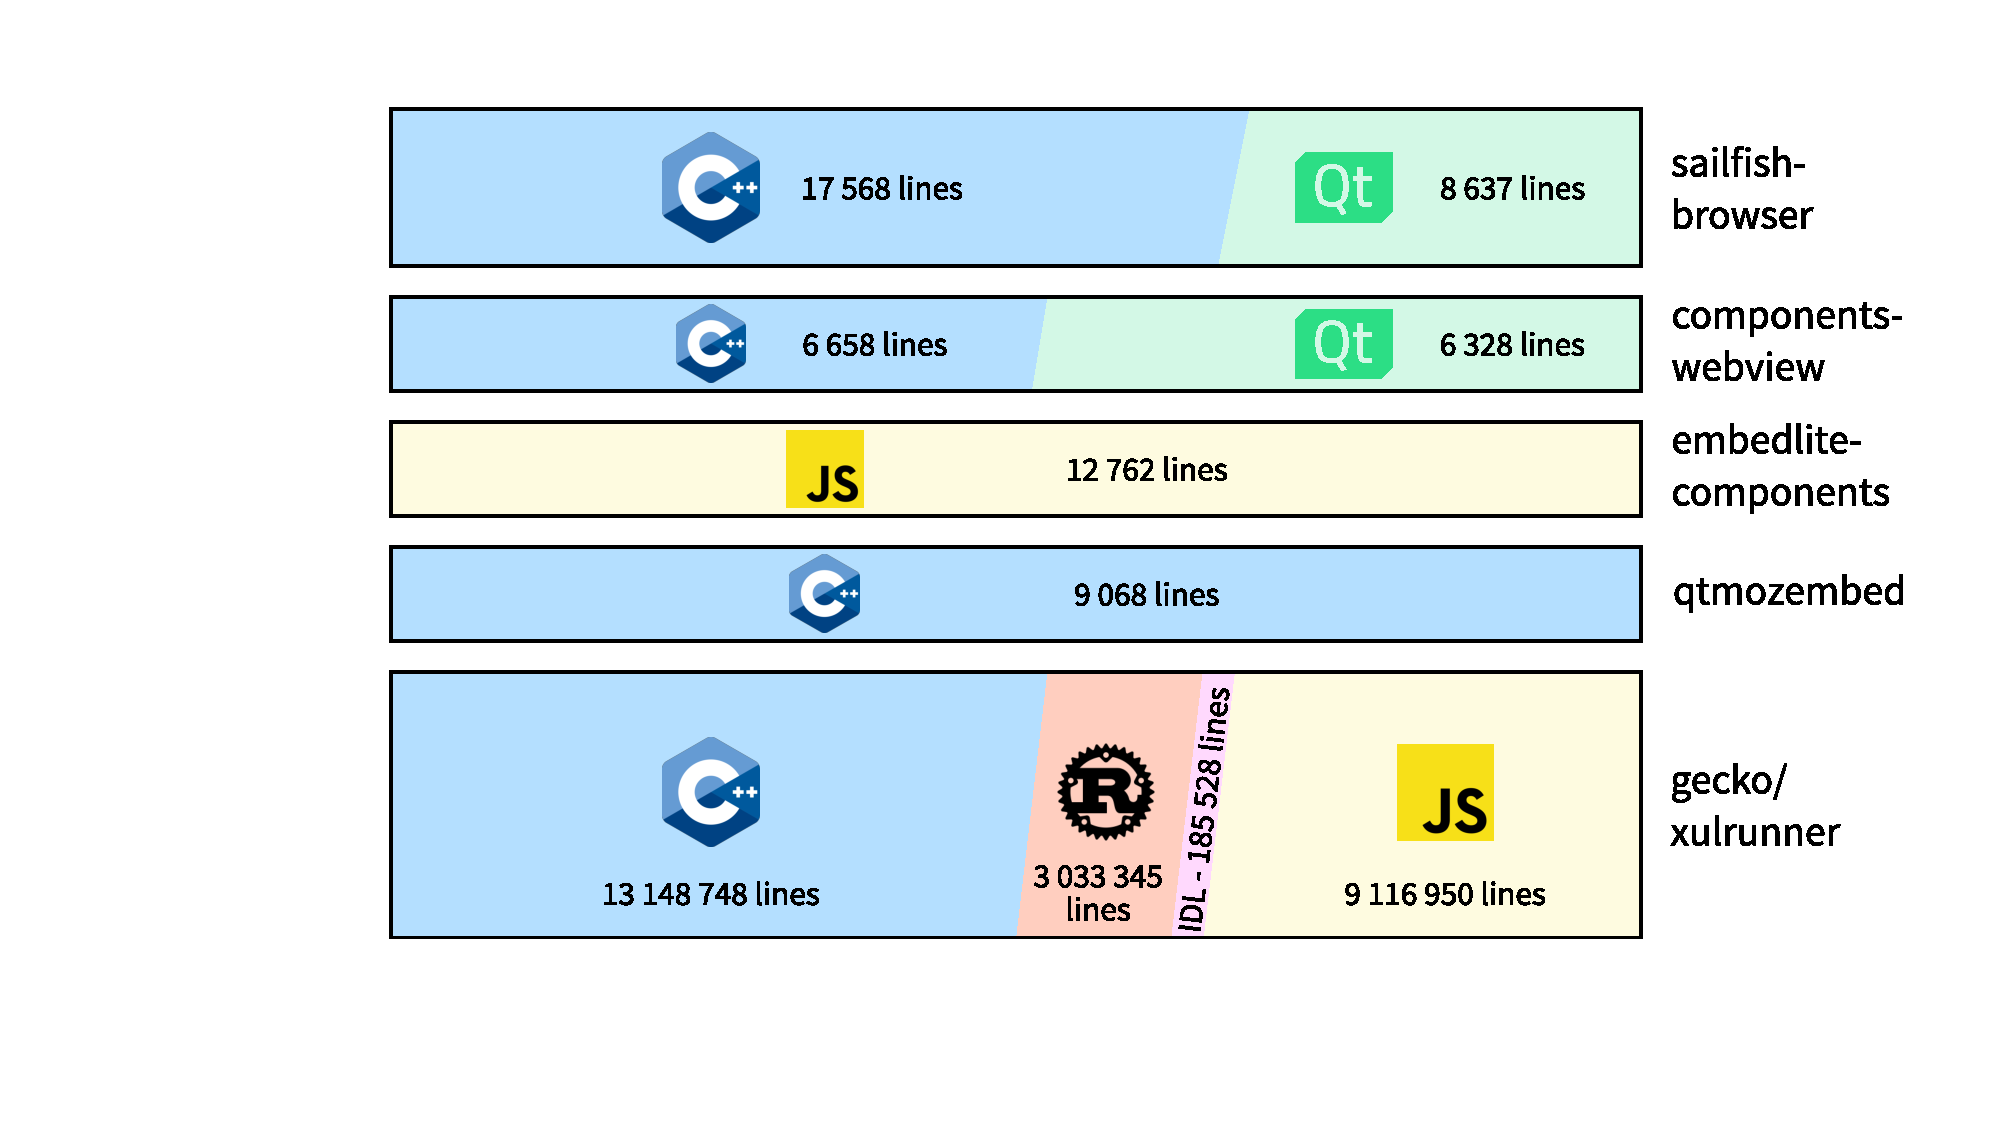
\includegraphics[width=1.0\textwidth]{components-languages}

\end{column}
\end{columns}

\end{frame}
\note{
\begin{enumerate}
\item The Sailfish Browser isn't just gecko.
\item {\tt sailfish-browser} provides the user interface (C++/Qt/QML).
\item {\tt embedlite-components} provides JavaScript user interface functionality (JavaScript).
\item {\tt qtmozembed} turns gecko into an embeddable Qt component (C++/Qt).
\item {\tt gecko} is the EmbedLite embedded gecko renderer (JavaScript/C++/Rust).
\end{enumerate}
}

%%%%%%%%%%%%%%%%%%%%%%%%%%%%%%%%%%%%%%%%%

\begin{frame}
\frametitle{Gecko Code Distribution}

\begin{columns}[T]
\begin{column}[T]{0.7\textwidth}

\vspace{0.5cm}
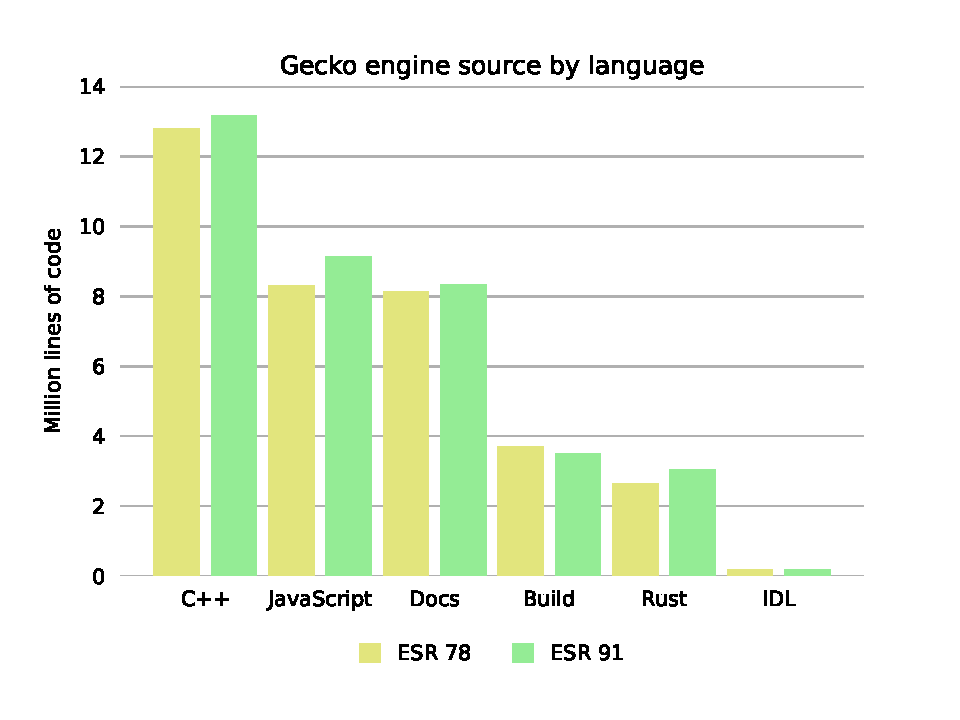
\includegraphics[width=1.0\textwidth]{totals}

\end{column}
\end{columns}

\end{frame}
\note{
\begin{enumerate}
\item -
\end{enumerate}
}

%%%%%%%%%%%%%%%%%%%%%%%%%%%%%%%%%%%%%%%%%

\begin{frame}
\frametitle{Chromium Code Distribution}

\begin{columns}[T]
\begin{column}[T]{0.7\textwidth}

\vspace{0.5cm}
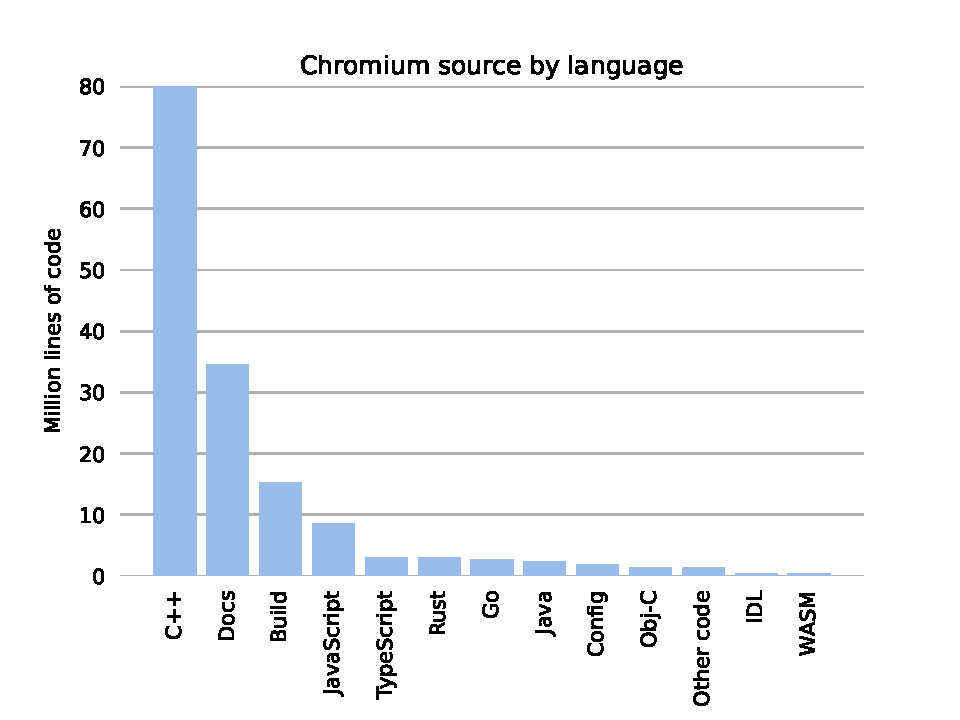
\includegraphics[width=1.0\textwidth]{totals-chromium}

\end{column}
\end{columns}

\end{frame}
\note{
\begin{enumerate}
\item -
\end{enumerate}
}

%%%%%%%%%%%%%%%%%%%%%%%%%%%%%%%%%%%%%%%%%

\begin{frame}
\frametitle{Gecko Patches}

\begin{columns}[T]
\begin{column}[T]{0.7\textwidth}

\vspace{0.5cm}
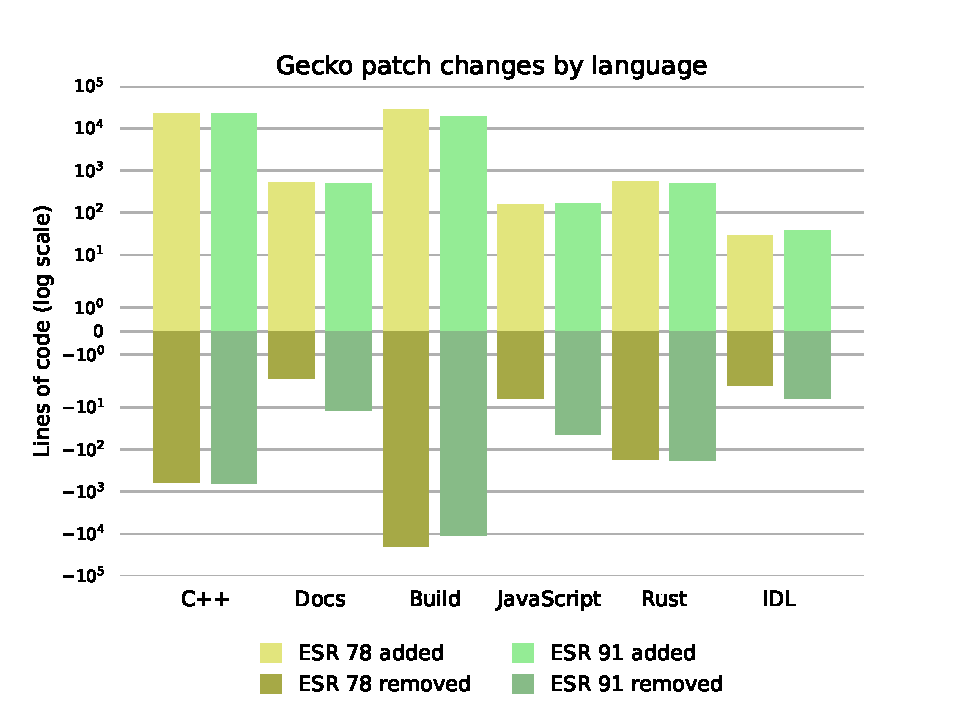
\includegraphics[width=1.0\textwidth]{patches}

\end{column}
\end{columns}

\end{frame}
\note{
\begin{enumerate}
\item -
\end{enumerate}
}

%%%%%%%%%%%%%%%%%%%%%%%%%%%%%%%%%%%%%%%%%

%\begin{frame}
%\frametitle{Dev Diary}

%\begin{columns}[T]
%\begin{column}[T]{0.6\textwidth}
%\setlength{\parskip}{0.5em}

%\vspace{1.2cm}
%{\huge
%\href{https://www.flypig.co.uk/gecko}{{\tt https:// \\
%www.flypig.co.uk \\
%/gecko\\
%}
%}}

%\end{column}
%\begin{column}[T]{0.3\textwidth}
%\setlength{\parskip}{0.5em}

%\vspace{0.5cm}
%
\includegraphics[width=1.0\textwidth]{qrcode-gecko-dev}

%\end{column}
%\end{columns}

%\end{frame}
%\note{
%}

%%%%%%%%%%%%%%%%%%%%%%%%%%%%%%%%%%%%%%%%%

\begin{frame}
\frametitle{Basic Browser Structure}

\begin{columns}[T]
\begin{column}[T]{0.66\textwidth}
\setlength{\parskip}{0.5em}

\vspace{1.5cm}
\begin{enumerate}
\setlength{\parskip}{0.5em}
\item Protocol client (HTTP/S, file, FTP,...)
\item JavaScript engine
\item Media decoder (JPG, PNG, audio, video)
\item DOM - Document Object Model
\item Layout/rendering engine (HTML, CSS, SVG)
\item Chrome
\end{enumerate}

\end{column}
\begin{column}[T]{0.34\textwidth}
\setlength{\parskip}{0.5em}

\vspace{-0.2cm}
\includegraphics[width=1.0\textwidth]{blocks}

\end{column}
\end{columns}

\end{frame}
\note{
\begin{enumerate}
\item -
\end{enumerate}
}

%%%%%%%%%%%%%%%%%%%%%%%%%%%%%%%%%%%%%%%%%

\begin{frame}
\frametitle{}

\begin{columns}[T]
\begin{column}[T]{1.0\textwidth}

\vspace{0.2cm}
\includegraphics[width=1.0\textwidth]{internals}

\end{column}
\end{columns}

\end{frame}
\note{
\begin{enumerate}
\item The internal building blocks of a browser and how they relate to one another.
\end{enumerate}
}

%%%%%%%%%%%%%%%%%%%%%%%%%%%%%%%%%%%%%%%%%

\begin{frame}
\frametitle{Embedded Browser Surface}

\begin{columns}[T]
\begin{column}[T]{0.7\textwidth}
\setlength{\parskip}{0.5em}

\vspace{1.0cm}
\begin{enumerate}
\setlength{\parskip}{0.5em}
\item Rendering canvas
\item Event loop and user input (taps, keyboard, APZ)
\item Browser actions
\item JavaScript in-DOM execution
\item JavaScript privileged execution
\item Message sending/receiving
\end{enumerate}

\end{column}
\begin{column}[T]{0.3\textwidth}
\setlength{\parskip}{0.5em}

\vspace{0.5cm}
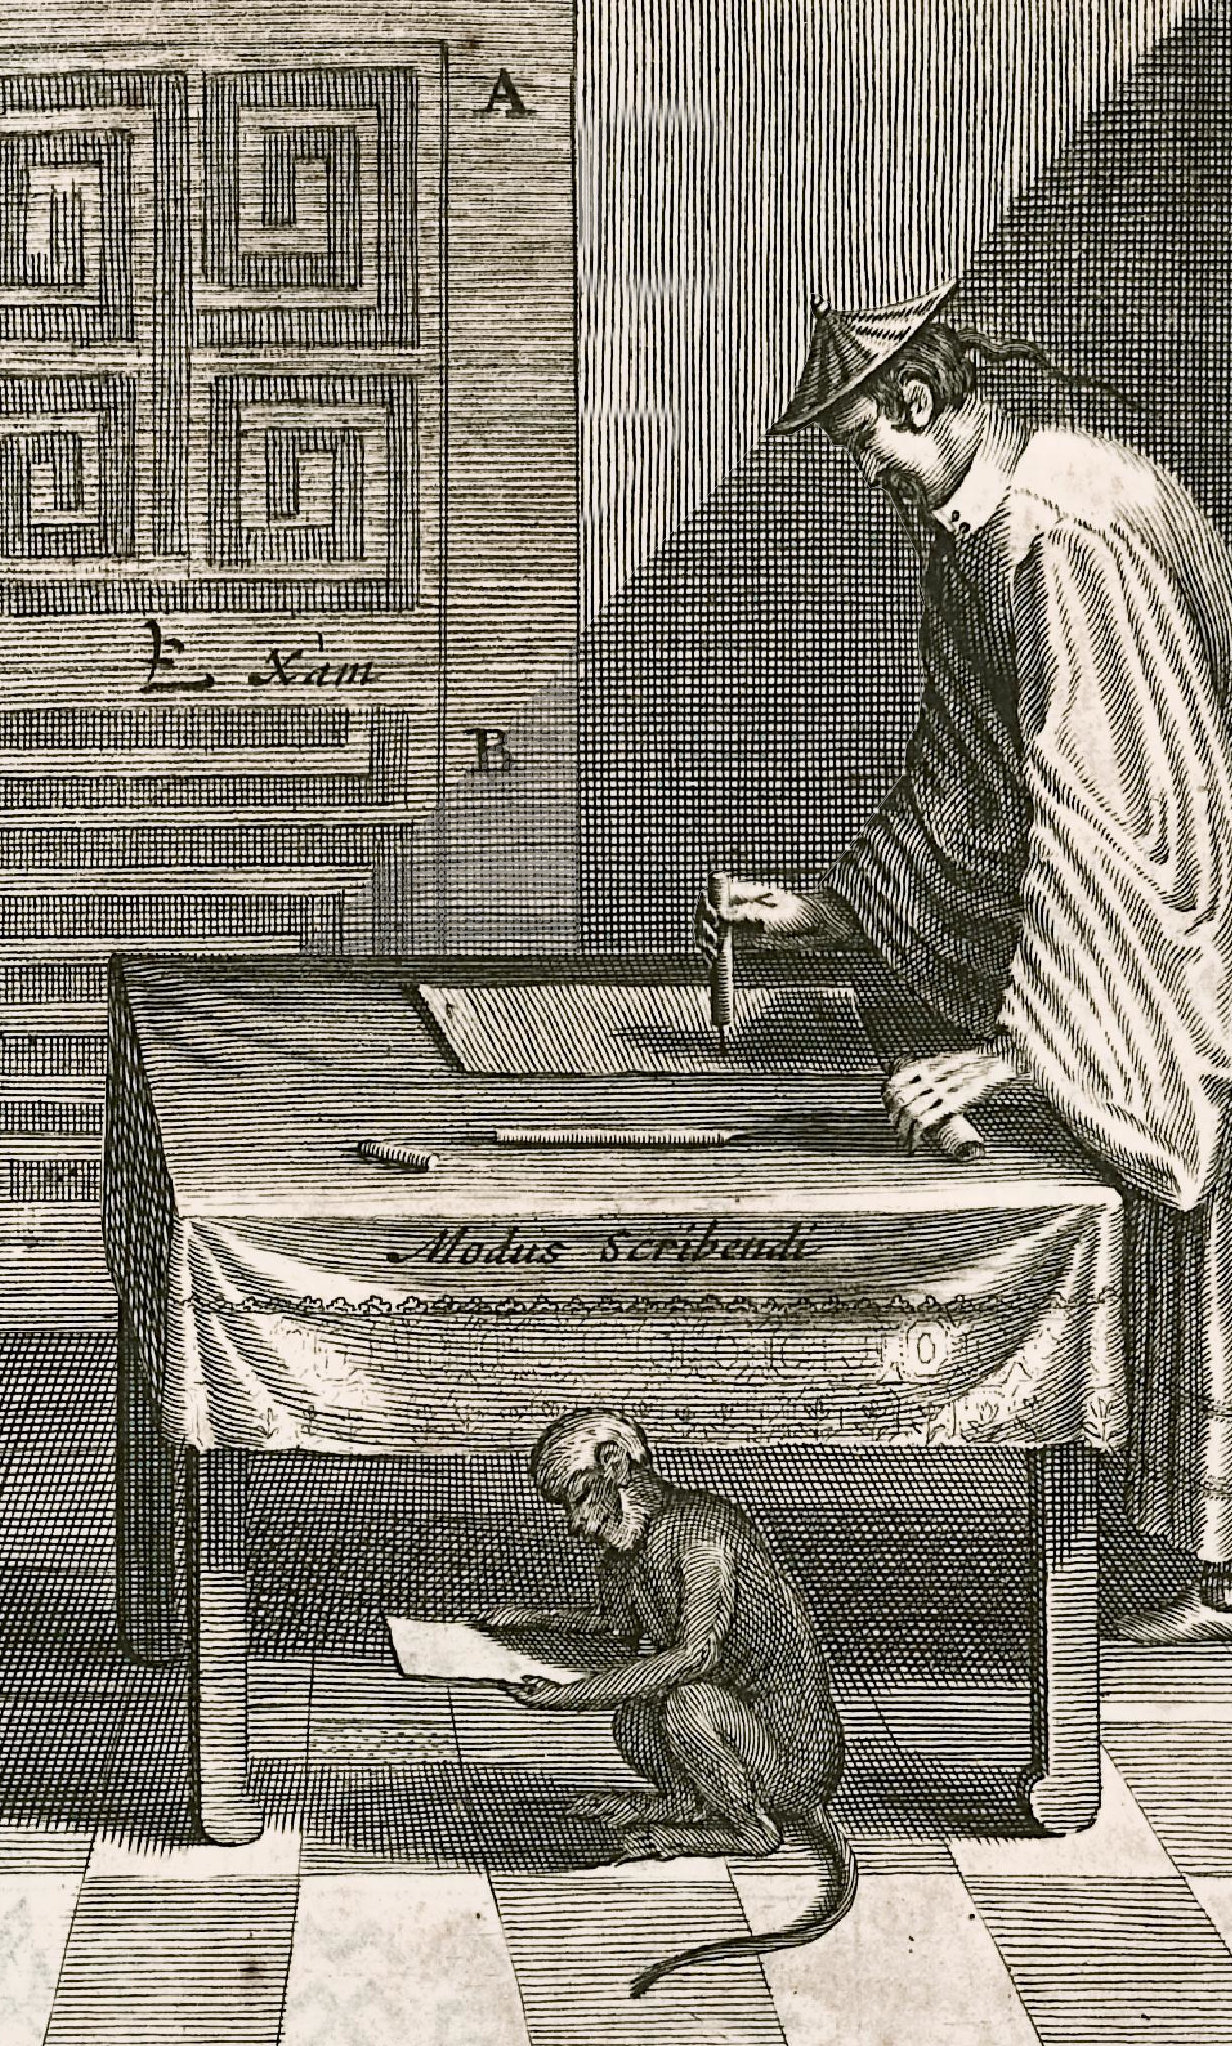
\includegraphics[width=0.8\textwidth]{chinese-room}

\end{column}
\end{columns}

\end{frame}
\note{
\begin{enumerate}
\item Image "Modus scribendi," National Library of Medicine, Illustration from p. 310 of Kircher's La Chine.
\item \url{http://resource.nlm.nih.gov/101595221}
\end{enumerate}
}

%%%%%%%%%%%%%%%%%%%%%%%%%%%%%%%%%%%%%%%%%

\begin{frame}
\frametitle{Emedding APIs}

\begin{columns}[T]
\begin{column}[T]{0.73\textwidth}
\setlength{\parskip}{0.5em}

\vspace{1.0cm}
Most browser embedding frameworks offer a similar API
\begin{enumerate}
\setlength{\parskip}{0.5em}
\item Settings controller
\item Javascript execution
\item Web controls (load, forwards, back)
\item Separate view widgets
\item Message passing interface
\end{enumerate}
Brief look at Chromium Embedded Framework, Sailfish WebView, QtWebEngine
\end{column}
\begin{column}[T]{0.2\textwidth}
\setlength{\parskip}{0.5em}

\vspace{0.5cm}
\hspace{-1.0cm}

\includegraphics[width=1.0\textwidth]{embedded-framework-logos}

\end{column}
\end{columns}

\end{frame}
\note{
\begin{enumerate}
\item -
\end{enumerate}
}

%%%%%%%%%%%%%%%%%%%%%%%%%%%%%%%%%%%%%%%%%

\begin{frame}
\frametitle{}

\begin{columns}[T]
\begin{column}[T]{0.5\textwidth}
\setlength{\parskip}{0.5em}

\vspace{0.7cm}

\lstinputlisting[language=cpp,firstline=1,lastline=24]{code-examples/blink-browser.cpp}

\end{column}
\begin{column}[T]{0.5\textwidth}
\setlength{\parskip}{0.5em}

\vspace{0.7cm}

\lstinputlisting[language=cpp,firstline=26,lastline=41]{code-examples/blink-browser.cpp}

\lstinputlisting[language=cpp,firstline=43,lastline=54]{code-examples/blink-browser.cpp}

\end{column}
\end{columns}

\end{frame}
\note{
\begin{enumerate}
\item -
\end{enumerate}
}

%%%%%%%%%%%%%%%%%%%%%%%%%%%%%%%%%%%%%%%%%

\begin{frame}
\frametitle{}

\begin{columns}[T]
\begin{column}[T]{0.5\textwidth}
\setlength{\parskip}{0.5em}

\vspace{0.4cm}

\lstinputlisting[language=cpp,firstline=1,lastline=21]{code-examples/blink-qtweb.cpp}

\end{column}
\begin{column}[T]{0.5\textwidth}
\setlength{\parskip}{0.5em}

\vspace{0.4cm}

\lstinputlisting[language=cpp,firstline=23,lastline=49]{code-examples/blink-qtweb.cpp}

\end{column}
\end{columns}

\end{frame}
\note{
\begin{enumerate}
\item -
\end{enumerate}
}

%%%%%%%%%%%%%%%%%%%%%%%%%%%%%%%%%%%%%%%%%

\begin{frame}
\frametitle{}

\begin{columns}[T]
\begin{column}[T]{0.5\textwidth}
\setlength{\parskip}{0.5em}

\vspace{0.5cm}

\lstinputlisting[language=cpp,firstline=1,lastline=18]{code-examples/gecko-webview.cpp}

\lstinputlisting[language=cpp,firstline=20,lastline=31]{code-examples/gecko-webview.cpp}

\end{column}
\begin{column}[T]{0.5\textwidth}
\setlength{\parskip}{0.5em}

\vspace{0.5cm}

\lstinputlisting[language=cpp,firstline=33,lastline=52]{code-examples/gecko-webview.cpp}

\end{column}
\end{columns}

\end{frame}
\note{
\begin{enumerate}
\item -
\end{enumerate}
}

%%%%%%%%%%%%%%%%%%%%%%%%%%%%%%%%%%%%%%%%%

\begin{frame}
\frametitle{Interface Definition Language}

\begin{columns}[T]
\begin{column}[T]{1.0\textwidth}
\setlength{\parskip}{0.5em}

\vspace{0.8cm}
\begin{enumerate}
\setlength{\parskip}{0.5em}
\item Interaction between native code and JavaScript
\item Requires type conversion and memory management
\item IDL - generate native/JS-compatible interfaces
\item Make native calls from JavaScript
\item Make JavaScript calls from native
\end{enumerate}
\end{column}
\end{columns}

\end{frame}
\note{
\begin{enumerate}
\item -
\end{enumerate}
}

%%%%%%%%%%%%%%%%%%%%%%%%%%%%%%%%%%%%%%%%%

\begin{frame}
\frametitle{}

\begin{columns}[T]
\begin{column}[T]{1.048\textwidth}
\setlength{\parskip}{0.5em}

\vspace{0.4cm}

\lstinputlisting[language=idl,firstline=4,lastline=16]{code-examples/prompt-factory.cpp}

\lstinputlisting[language=cpp,firstline=102,lastline=113]{code-examples/prompt-factory.cpp}

\end{column}
\end{columns}

\end{frame}
\note{
\begin{enumerate}
\item -
\end{enumerate}
}

%%%%%%%%%%%%%%%%%%%%%%%%%%%%%%%%%%%%%%%%%

\begin{frame}
\frametitle{}

\begin{columns}[T]
\begin{column}[T]{0.5\textwidth}
\setlength{\parskip}{0.5em}

\vspace{0.5cm}

\lstinputlisting[language=JavaScript,firstline=21,lastline=49]{code-examples/prompt-factory.cpp}

\end{column}
\begin{column}[T]{0.5\textwidth}
\setlength{\parskip}{0.5em}

\vspace{0.5cm}

\lstinputlisting[language=cpp,firstline=119,lastline=147]{code-examples/prompt-factory.cpp}

\end{column}
\end{columns}

\end{frame}
\note{
\begin{enumerate}
\item -
\end{enumerate}
}

%%%%%%%%%%%%%%%%%%%%%%%%%%%%%%%%%%%%%%%%%

\begin{frame}
\frametitle{}

\begin{columns}[T]
\begin{column}[T]{1.048\textwidth}
\setlength{\parskip}{1.048em}

\vspace{0.5cm}

\lstinputlisting[language=JavaScript,firstline=71,lastline=84]{code-examples/prompt-factory.cpp}

\lstinputlisting[language=cpp,firstline=55,lastline=66]{code-examples/prompt-factory.cpp}

\end{column}
\end{columns}

\end{frame}
\note{
\begin{enumerate}
\item -
\end{enumerate}
}

%%%%%%%%%%%%%%%%%%%%%%%%%%%%%%%%%%%%%%%%%

\begin{frame}
\frametitle{XULRunner}

\begin{columns}[T]
\begin{column}[T]{0.5\textwidth}
\setlength{\parskip}{0.5em}

\vspace{1.5cm}
What is xulrunner?
\begin{enumerate}
\setlength{\parskip}{0.5em}
\item XUL: XML User interface Language
\item xulrunner: build process to generate a library
\item Officially deprecated in 2016
\item Outputs libxul.so and related artefacts
\end{enumerate}

\end{column}
\begin{column}[T]{0.5\textwidth}
\setlength{\parskip}{0.5em}

\vspace{0.5cm}

\includegraphics[width=1.0\textwidth]{mozilla}

\end{column}
\end{columns}

\end{frame}
\note{
\begin{enumerate}
\item -
\end{enumerate}
}

%%%%%%%%%%%%%%%%%%%%%%%%%%%%%%%%%%%%%%%%%

\begin{frame}
\frametitle{EmbedLite}

\begin{columns}[T]
\begin{column}[T]{0.5\textwidth}
\setlength{\parskip}{0.5em}

\vspace{1.5cm}
What is xulrunner?
\begin{enumerate}
\setlength{\parskip}{0.5em}
\item XULRunner with hooks for Qt event loop support
\item Run as a thread or a process
\end{enumerate}

\end{column}
\begin{column}[T]{0.5\textwidth}
\setlength{\parskip}{0.5em}

\vspace{0.5cm}

\includegraphics[width=1.0\textwidth]{mozilla}

\end{column}
\end{columns}

\end{frame}
\note{
\begin{enumerate}
\item -
\end{enumerate}
}

%%%%%%%%%%%%%%%%%%%%%%%%%%%%%%%%%%%%%%%%%

\begin{frame}
\frametitle{libxul.so}

\begin{columns}[T]
\begin{column}[T]{0.5\textwidth}
\setlength{\parskip}{0.5em}

\vspace{1.5cm}
\begin{enumerate}
\setlength{\parskip}{0.5em}
\item Provides HTTP client, renderer, JavaScript interpretter
\item Everything except the front-end
\item Methods for sending and receiving IPC calls
\item Exposes the full Gecko interface
\item Including calls to register privileged JavaScript
\end{enumerate}

\end{column}
\begin{column}[T]{0.5\textwidth}
\setlength{\parskip}{0.5em}

\vspace{0.5cm}

\includegraphics[width=1.0\textwidth]{mozilla}

\end{column}
\end{columns}

\end{frame}
\note{
\begin{enumerate}
\item -
\end{enumerate}
}

%%%%%%%%%%%%%%%%%%%%%%%%%%%%%%%%%%%%%%%%%

\begin{frame}
\frametitle{DocShell}

\begin{columns}[T]
\begin{column}[T]{0.5\textwidth}
\setlength{\parskip}{0.5em}

\vspace{1.5cm}
\begin{enumerate}
\setlength{\parskip}{0.5em}
\item -
\end{enumerate}

\end{column}
\begin{column}[T]{0.5\textwidth}
\setlength{\parskip}{0.5em}

\vspace{0.5cm}

\includegraphics[width=1.0\textwidth]{mozilla}

\end{column}
\end{columns}

\end{frame}
\note{
\begin{enumerate}
\item -
\end{enumerate}
}

%%%%%%%%%%%%%%%%%%%%%%%%%%%%%%%%%%%%%%%%%

\begin{frame}
\frametitle{DOMWindow}

\begin{columns}[T]
\begin{column}[T]{0.5\textwidth}
\setlength{\parskip}{0.5em}

\vspace{1.5cm}
\begin{enumerate}
\setlength{\parskip}{0.5em}
\item -
\end{enumerate}

\end{column}
\begin{column}[T]{0.5\textwidth}
\setlength{\parskip}{0.5em}

\vspace{0.5cm}

\includegraphics[width=1.0\textwidth]{mozilla}

\end{column}
\end{columns}

\end{frame}
\note{
\begin{enumerate}
\item -
\end{enumerate}
}

%%%%%%%%%%%%%%%%%%%%%%%%%%%%%%%%%%%%%%%%%

\begin{frame}
%\frametitle{Thigg's Images}

\begin{columns}[T]
\begin{column}[T]{1.0\textwidth}

\vspace{-0.12cm}
\hspace*{-1.1cm}
\includegraphics[width=1.15\textwidth]{Thigg}

\end{column}
\end{columns}

\end{frame}
\note{
\begin{enumerate}
\item A special shout-out to Thigg who has been created AI-generated images to go alongside my blog posts. They are amazing.
\end{enumerate}
}

%%%%%%%%%%%%%%%%%%%%%%%%%%%%%%%%%%%%%%%%%

\begin{frame}[fragile]
\frametitle{Further info}
\setlength{\leftmargini}{7.5em}
\vspace{1.0cm}

\begin{itemize}
\setlength{\parskip}{1.0em}
\item[Dev Diary \,] \url{https://www.flypig.co.uk/gecko}
\item[Slides source \,] \url{https://github.com/llewelld/techtalk-gecko-dev}
\item[Gecko source \,] \url{https://github.com/llewelld/gecko-dev}
\item[CEF \,] \url{https://bitbucket.org/chromiumembedded/cef}
\item[QtWebEngine \,] \url{https://doc.qt.io/qt-6/qtwebengine-index.html}
\item[WebView \,] \url{https://sailfishos.org/develop/docs/sailfish-components-webview}
\end{itemize}

\end{frame}
\note{
\fontsize{7pt}{8pt}{\bibliographystyle{ieeetr}}
\bibliography{slides}
}

%%%%%%%%%%%%%%%%%%%%%%%%%%%%%%%%%%%%%%%%%

\end{document}
